\documentclass{beamer}

\mode<presentation>
{
  \usetheme{Montpellier}
  \usecolortheme{beaver}
  \setbeamercovered{transparent}
}

\usepackage[english]{babel}
\usepackage[latin1]{inputenc}
\usepackage{times}
\usepackage[T1]{fontenc} 
% Or whatever. Note that the encoding and the font should match. If T1
% does not look nice, try deleting the line with the fontenc.
\usepackage{amsmath}
\newcommand{\linespace}{\vskip 0.25cm}

\definecolor{MyForestGreen}{rgb}{0,0.7,0} 
\newcommand{\tableemph}[1]{{#1}}
\newcommand{\tablewin}[1]{\tableemph{#1}}
\newcommand{\tablemid}[1]{\tableemph{#1}}
\newcommand{\tablelose}[1]{\tableemph{#1}}

\definecolor{MyLightGray}{rgb}{0.6,0.6,0.6}
\newcommand{\tabletie}[1]{\color{MyLightGray} {#1}}

% The text in square brackets is the short version of your title and will be used in the
% header/footer depending on your theme.
\title[Thermal Interaction In SAR]{Thermal Interaction in \\ Spatial Augmented Reality}

% Sub-titles are optional - uncomment and edit the next line if you want one.
% \subtitle{Why does sub-tree crossover work?} 

% The text in square brackets is the short version of your name(s) and will be used in the
% header/footer depending on your theme.
\author[YaDeau]{Justin Brennen YaDeau}

% The text in square brackets is the short version of your institution and will be used in the
% header/footer depending on your theme.
\institute[U of Minn, Morris]
{
  Division of Science and Mathematics \\
  University of Minnesota, Morris \\
  Morris, Minnesota, USA
}

% The text in square brackets is the short version of the date if you need that.
\date[December '15] % (optional)
{5 December 2015}

% Delete this, if you do not want the table of contents to pop up at
% the beginning of each subsection:
\AtBeginSection[]
{
  \begin{frame}<beamer>
    \frametitle{Outline}
    \tableofcontents[currentsection, hideothersubsections]
  \end{frame}
}

\begin{document}

\begin{frame}
  \titlepage
\end{frame}

% For a 20-25 minute senior seminar talk you probably want something like:
% - Two or three major sections (other than the summary).
% - At *most* three subsections per section.
% - Talk about 30s to 2min per frame. So there should probably be between
%   15 and 30 frames, all told.

\section*{Overview}

\subsection*{Background}

\begin{frame}

  \frametitle{Background}
  
  \begin{columns}
  \begin{column}{0.6\textwidth}
  \begin{itemize}
  	\item Virtual Reality
	\item Augmented Reality
	\item Spatial Augmented Reality
	\item 6DOF
  \end{itemize}
  \end{column}
  \end{columns}
\end{frame}

\begin{frame}
	\frametitle{Virtual Reality}
	\begin{itemize}
		\item Completely Virtual
		\item The Matrix 
		\item Oculus Rift
	\end{itemize}
\end{frame}

\begin{frame}
	\frametitle{Augmented Reality}
	
	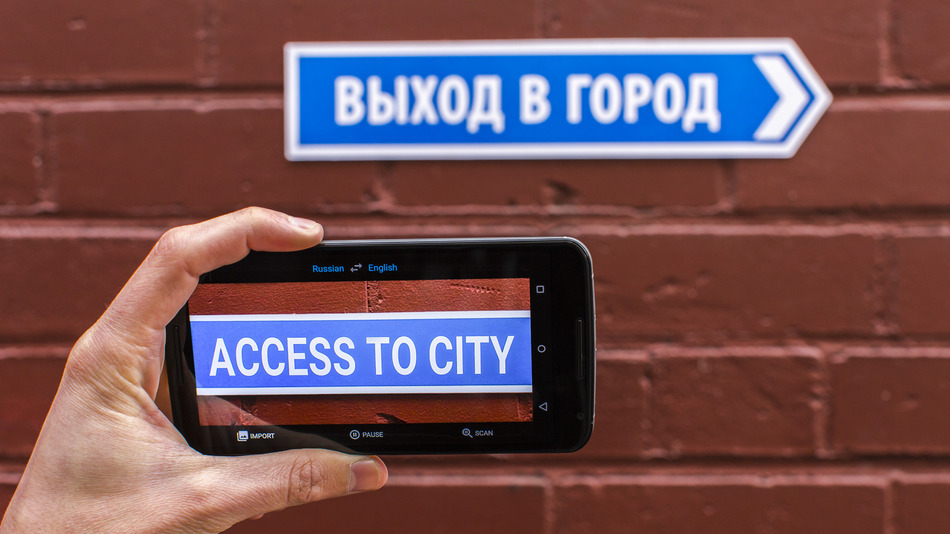
\includegraphics[width=\textwidth]{images/google-translate}
\end{frame}

\begin{frame}
	\frametitle{Spatial Augmented Reality}
\end{frame}

\begin{frame}
	\frametitle{6DOF}
	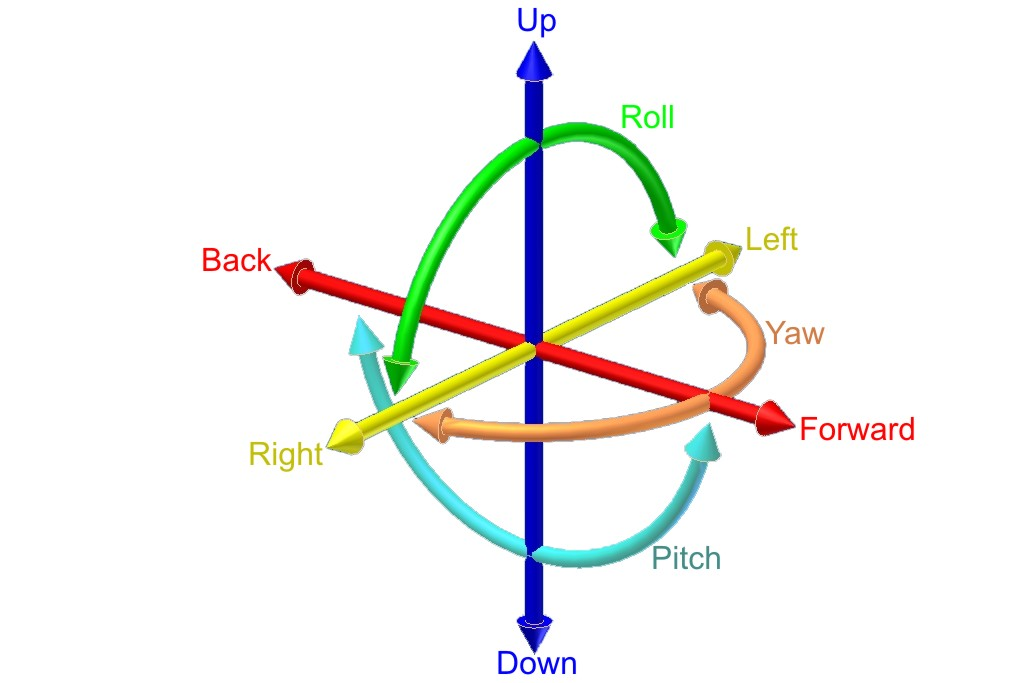
\includegraphics[width=\textwidth]{../Sample_paper/images/6DOF_en}
\end{frame}

\subsection*{Outline}
\begin{frame}
  \frametitle{Outline}
  \tableofcontents[hideallsubsections]
\end{frame}

\section[Mobile Thermal Interaction]{Thermal interaction with mobile devices}

\subsection{Hardware}
\begin{frame}
\frametitle{Hardware}	

	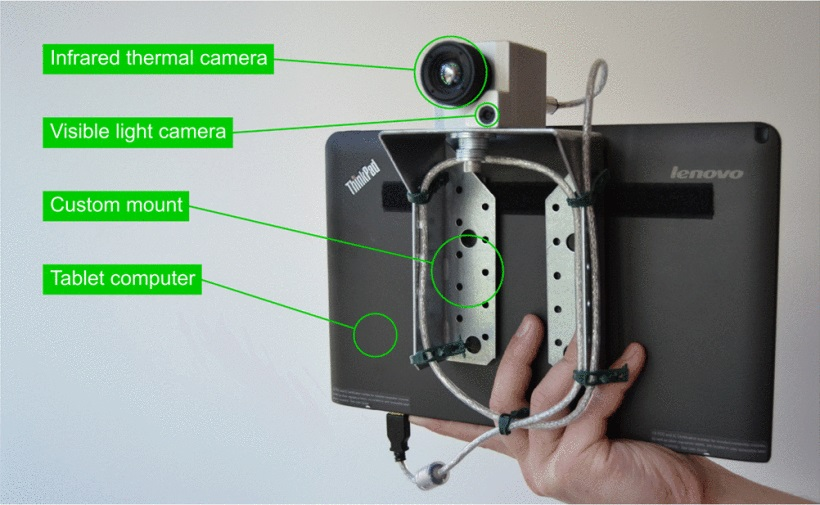
\includegraphics[width=\textwidth]{../Sample_paper/images/Hardware2}
	
\end{frame}

\subsection{Thermal Detection}
\begin{frame}
\frametitle{Thermal Detection}
	\begin{itemize}
		\item Assumes a controlled environment
		\item Object-only, hand-only, obstruction-by-hand, and touch-by-hand
		\item Interactions leave thermal impressions on the object
		\item Using the OpenCV SimpleBlobDetector
	\end{itemize}
\end{frame}

\begin{frame}
\frametitle{OpenCV SimpleBlobDetector}
	\begin{itemize}
		\item 
	\end{itemize}
\end{frame}

\subsection{Object Tracking}
\begin{frame}	
\frametitle{Object Tracking}
\end{frame}

\subsection{Materials Tested}
\begin{frame}	
\frametitle{Materials Tested}
\end{frame}



\subsection{Applications}

\begin{frame}
	\frametitle{Applications}
	Applications that use thermal imaging with mobile technology 
	\begin{itemize}
		\item "Spray on" graphical user interfaces (GUI)
		\item Augmented floor plans
	\end{itemize}
\end{frame}

\begin{frame}
	\frametitle{"Spray on" GUIs}	
	\begin{columns}
	\begin{column}{0.45\textwidth}
	\begin{itemize}
		\item The screen displays a dial pad, but there is no dial pad on the surface
		\item Looking at the screen to interact with dial pad
		\item Devices without touch screens
	\end{itemize}		
	\end{column}
	\begin{column}{0.55\textwidth}
	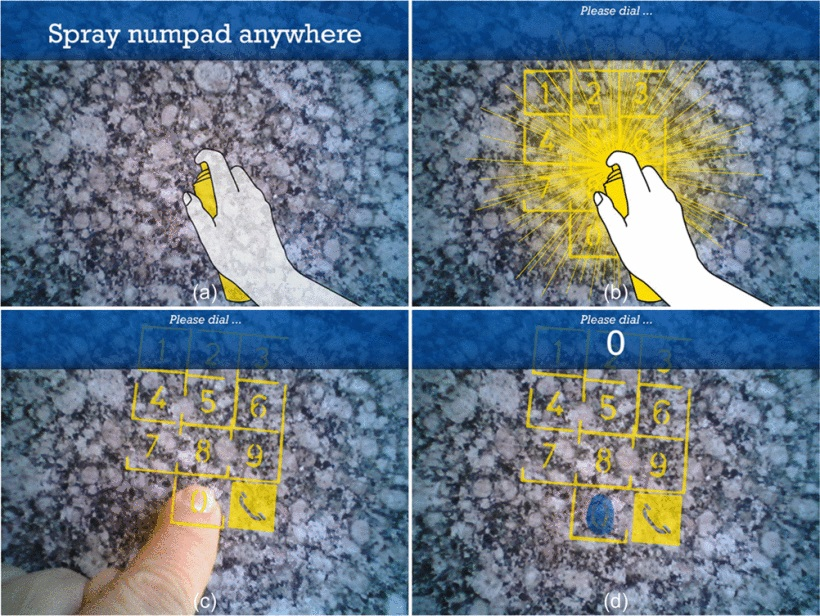
\includegraphics[width=\textwidth]{../Sample_paper/images/numpad}
	\end{column}
	\end{columns}
\end{frame}

\begin{frame}
	\frametitle{Augmented Floor Plans}
	\begin{columns}
	\begin{column}{0.45\textwidth}
	\begin{itemize}
		\item Similar interaction, different interface
		\item Using number sections as buttons
	\end{itemize}
	\end{column}
	\begin{column}{0.55\textwidth}
	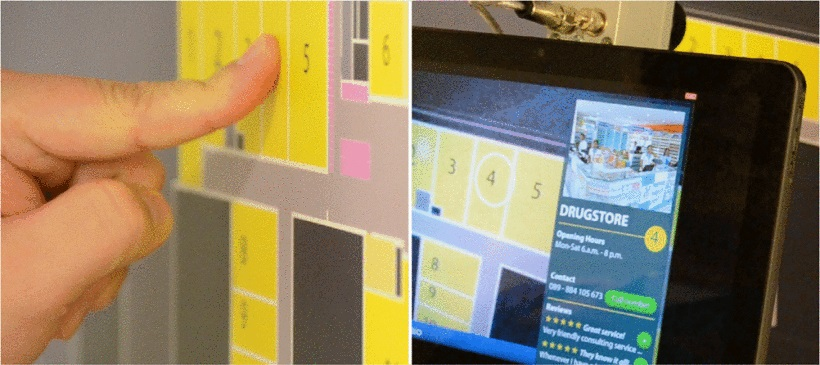
\includegraphics[width=\textwidth]{images/AugmentedFloorPlans}
	\end{column}
	\end{columns}
	
\end{frame}

\section[Using spatial augmented reality for 3D data visualization]{Using spatial augmented reality for 3D data visualization}

\subsection{Visualizing Data}
\begin{frame}	
\frametitle{Visualizing Data}
	\begin{itemize}
		\item Representing data visually
		\item Examples: weather maps, pie and bar charts, etc
		\item The importance of visualizing data
	\end{itemize}
\end{frame}

\subsection{Applications}
\begin{frame}
\frametitle{Applications}
	Applications that use spatial augmented reality for 3D data visualization   
	\begin{itemize}
		\item Table-Top
		\item CAVE
	\end{itemize}
\end{frame}

\begin{frame}
\frametitle{Table-Top} 
	\begin{itemize}
		\item Using a hand held pointing device a user can zoom in or out of the visualization 
		\item The interactions happen inside the virtual volume
	\end{itemize}
\end{frame}

\begin{frame}
\frametitle{Table-Top} 
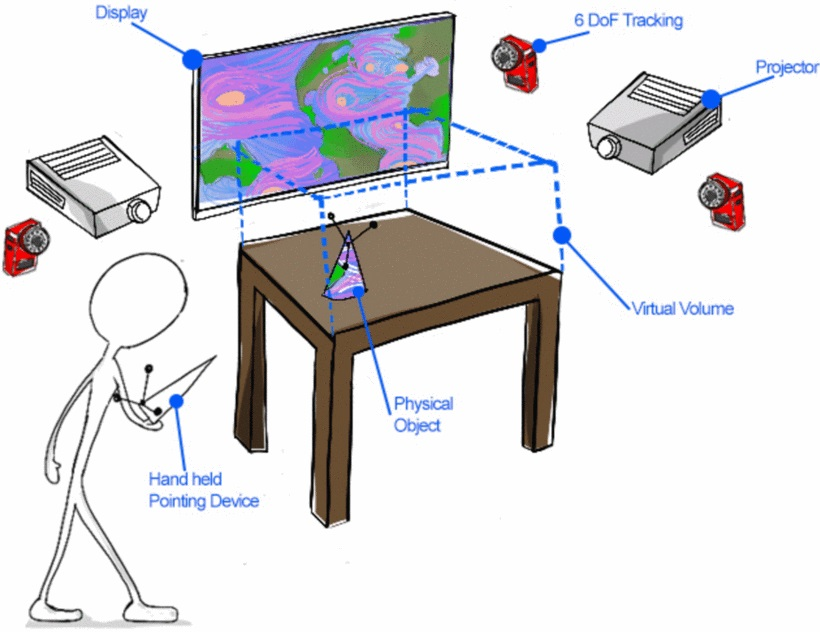
\includegraphics[width=\textwidth]{../Sample_paper/images/Tabletop}
\end{frame}

\begin{frame}
\frametitle{CAVE}
	\begin{itemize}
		\item Larger area than the table-top method
		\item Increase in collaborators/viewers
		\item Similar interactions as the table-top method
	\end{itemize}
\end{frame}

\begin{frame}
\frametitle{CAVE}
\includegraphics[width=\textwidth]{../Sample_paper/images/CAVE}
\end{frame}

\subsection{Limitations}
\begin{frame}	
\frametitle{Limitations}
	\begin{itemize}
		\item Strength of the projectors 
		\item Needing a controlled environment 
		\item Solutions
	\end{itemize}
\end{frame}

\section[Conclusions]{Conclusions}
\begin{frame}
\frametitle{Conclusions}
	\begin{itemize}
		\item 
	\end{itemize}
\end{frame}

\begin{frame}
	\frametitle{Thanks!}
	
	Thank you for your time and attention!
		
	\linespace
	\linespace
	
	Contact:  
	\begin{itemize}
		\item \texttt{yadea003@morris.umn.edu}
	\end{itemize}
	
	\linespace
	\linespace
	
	\begin{center}
	{\huge Any Questions?}
	\end{center}
\end{frame}

\end{document}


